\documentclass[12pt]{article}

\usepackage[utf8]{inputenc}
\usepackage{graphicx}
\usepackage{fancyhdr}

\title{g55\_RANDU - Generate Pseudorandom Number with IBM RANDU Parameters}
\author{Group 55\\Juliette Regimbal (260657238)\\Qingzhou Yang (260687570)}
\date{February 20, 2017}
\pagenumbering{gobble}
\pagenumbering{arabic}
\pagestyle{fancy}

\begin{document}
\maketitle
\setlength{\parindent}{0ex}
\lhead{Group 55}
\rhead{Juliette Regimbal (260657238)\\Qingzhou Yang (260687570)}

\section{Circuit Description}
The \textit{g55\_RANDU} circuit is based on the IBM RANDU function, computing a pseudorandom number based on the formula $R = mod(a*SEED+b, c)$ where a, b, and c are constants, R is the pseudorandom number, and SEED is an initial value. The math involved is broken down into addition and bit shifting, with addition done using the \textit{lpm\_add\_sub} circuit provided in the Altera LPM library. The SEED input and R output are both 32-bit unsigned integers.\\
\begin{figure}[h!t]
\centering
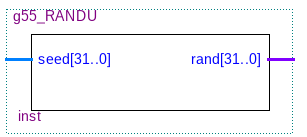
\includegraphics[scale=0.5]{graphics/randu_pinout.png}
\caption{\textit{g55\_RANDU} Pinout}
\end{figure}\\
The constants are 65539, 0, and $2^{31}$ for a, b, and c respectively. The value for a is equivalent to $10000000000000011_2$, so the operation $a*SEED$ only requires three additions and two shifts. As $mod(x, y) = x - floor(x/y)*y$ and in our case $c = 2^{31}$, two shift operations or setting all bits from the 29th to the 0th to 0 is necessary. Inversion and one addition operation is needed to calculate the two's complement, and then one more addition operation is needed to get a final value for R. So altogether 4 32-bit adders are necessary in the \textit{g55\_RANDU} circuit.\\

\section{Testing}
As testing all $2^{32}$ possible inputs is time consuming, only 5 inputs were tested. The first input was 1, with each successive input being the output of the previous test. For example, if input $i_{n-1}$ yields output $o_{n-1}$, then the next input $i_n = o_{n-1}$. Since the RANDU function is well known, the relationship between three pseudorandom numbers $R_n$, $R_{n-1}$, and $R_{n-2}$ is that $mod(R_n - 6 * R_{n-1} + 9 * R_{n-2}, 2^{31}) = 0$. If the generated numbers have this relationship, then the \textit{g55\_RANDU} circuit works properly.\\

\begin{figure}[h!t]
\centering
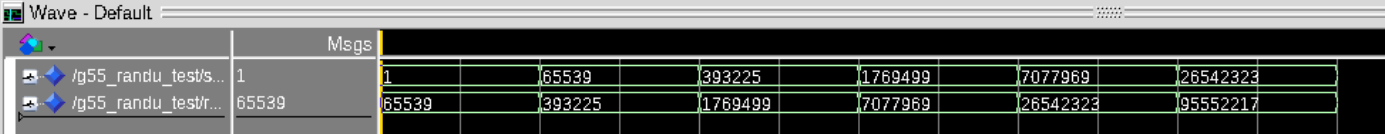
\includegraphics[scale=0.3]{graphics/randu_wave2.png}
\caption{\textit{g55\_RANDU} Waveform}
\end{figure}

The outputs in order are 65539, 393225, 1769499, 7077969, 26542323, and 95552217. They were put into matlab to verify that the relationship holds, and the modulo comes out to be 0. Based on this, we know the random number generator is working as expected.

\end{document}